%/*******************************************************************************
% * Copyright (c) 2009, A. Kaufmann and Elexis
% * All rights reserved. This program and the accompanying materials
% * are made available under the terms of the Eclipse Public License v1.0
% * which accompanies this distribution, and is available at
% * http://www.eclipse.org/legal/epl-v10.html
% *
% * Contributors:
% *    A. Kaufmann - initial implementation
% *
% * $Id: MesswertBase.java 5386 2009-06-23 11:34:17Z rgw_ch $
% *******************************************************************************/

\documentclass[a4paper]{scrartcl}
\usepackage{german}
\usepackage[utf8]{inputenc}
\usepackage[german]{babel}
\usepackage[]{hyperref}
\usepackage{listings}
\usepackage{booktabs}
\usepackage[pdftex]{graphicx}

\lstset{extendedchars=false}

\title{Hilotec-Messwerte}
\author{Antoine Kaufmann}

\begin{document}
\maketitle
\section{Einführung}
Dieses Elexis-Plugin ist dazu gedacht, Messungen und andere Erhebungsdaten in
Elexis strukturiert zu erfassen und zu verarbeiten. Mit dem Plugin
\textit{hilotec-pluginstatistiken} wird es auch ermöglicht, Auswertungen
darüber zu erstellen, und die Werte zu exportieren als CSV.

Das Plugin stellt eine View zur Verfügung, die eine Übersicht über alle
Messungen eines Patienten bietet, wo auch Neue Erfasst und Bestehende gelöscht
oder verändert werden können.

Die Konfiguration der möglichen Messungen und deren Struktur wird in einer
XML-Datei spezifiziert.


\section{Voraussetzungen}
\begin{itemize}
    \item Elexis 2.0
\end{itemize}

\section{Konfiguration}
Wie weiter oben bereits erwähnt, wird das Plugin über eine XML-Datei
konfiguriert. Diese Dateien befinden sich im Benutzerdatenverzeichnis von
Elexis:
\begin{description}
    \item[Windows:] \texttt{C:\textbackslash
                                Dokumente und Einstellungen\textbackslash
                                Benutzer\textbackslash Elexis\textbackslash
                                messwerte.xml}
    \item[Linux:] \texttt{/home/benutzer/elexis/messwerte.xml}
    % TODO: Mac?
\end{description}

Die verfügbaren Messungstypen werden mit \texttt{datatype}-Elementen im
Rootelement \texttt{datatypes} Deklariert. Pro Messungstyp kann ein Name, der
intern(unter anderem auch für die IDataAccess-Schnittstelle) zur Identifikation
des Typs benutzt wird, dieser kann mit dem Attribut \texttt{name} festgelegt
werden. Die Messungsbezeichnung, die dem Benutzer angezeigt wird, kann über das
Attribut \texttt{title} konfiguriert werden. In der XML Datei sieht das
folgendermassen aus:
\begin{lstlisting}
<?xml version="1.0">
<datatypes>
  <datatype name="masse" title="Masse">
    <numfield name="gewicht" title="Gewicht" unit="kg" />
    <numfield name="groesse" title="Groesse" unit="m" />
  </datatype>
  <datatype name="bdruck" title="Blutdruck">
    <numfield name="bdsys" title="Systolisch" unit="mm Hg" />
    <numfield name="bddia" title="Diastolisch" unit="mm Hg" />
  </datatype>
</datatypes>
\end{lstlisting}

In den \texttt{datatype}-Tags können die zur Messung gehörenden Felder
eingetragen werden.

Bei allen Feldtypen sind die folgenden Attribute verfügbar:
\begin{description}
    \item[name:] Interner Feldname, muss eindeutig sein in dem Typ
    \item[title:] Dem Benutzer angezeigter Titel
    \item[unit:] Einheit(nur für den Benutzer)
\end{description}

Im Folgenden wird auf die einzelnen Feldtypen genauer eingegangen. Die
angegebenen Typnamen sind gleichzeitig auch die XML-Tagnamen um Felder des
entsprechenden


\subsection{strfield}
Ein- oder mehrzeiliges Textfeld
\begin{center}
    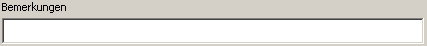
\includegraphics[width=12cm]{images/strfield.png}
\end{center}
\subsubsection{Attribute}
\begin{description}
    \item [default:] Standardwert, wenn die Messung neu erfasst wird
    \item [lines:] Anzahl Zeilen des Textfeldes \textit([Standard: 1])
\end{description}
\subsection{Beispiel}
\begin{lstlisting}
<strfield name="bemerk" title="Bemerkungen" lines="5" />
\end{lstlisting}


\subsection{numfield}
Zahlenfeld
\begin{center}
    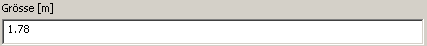
\includegraphics[width=12cm]{images/numfield.png}
\end{center}
\subsubsection{Attribute}
\begin{description}
    \item [default:] Standardwert, wenn die Messung neu erfasst wird
\end{description}
\subsection{Beispiel}
\begin{lstlisting}
<numfield name="gewicht" title="Gewicht" unit="kg" />
\end{lstlisting}

\subsection{scalefield}
Feld um Ganzzahlen in einem bestimmten Bereich zu erfassen
\begin{center}
    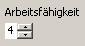
\includegraphics[width=2.3cm]{images/scalefield.png}
\end{center}
\subsubsection{Attribute}
\begin{description}
    \item[default:]  Standardwert, wenn die Messung neu erfasst wird
    \item[min:] Kleinster erfassbarer Wert
    \item[max:] Grösster erfassbarer Wert
\end{description}
\subsection{Beispiel}
\begin{lstlisting}
<scalefield name="arfaeh" title="Arbeitsfaehigkeit"
  min="0" max="5" default="5" />
\end{lstlisting}

\subsection{enumfield}
Auswahlfeld mit einer fixen Liste an Auswahlmöglichkeiten
\begin{center}
    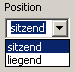
\includegraphics[width=2.2cm]{images/enumfield.png}
\end{center}
\subsubsection{Attribute}
\begin{description}
    \item[default:] Standardwert, wenn die Messung neu erfasst wird. Muss
                    angegeben werden und dem Wert einer Option aus der Liste
                    entsprechen.
\end{description}
\subsubsection{Unterelemente}
Die einzelnen auswählbaren Optionen werden mit dem Unterlement \texttt{option}
spezifiziert. Für jede Option muss ein interner Wert mit dem Attribut
\texttt{value} angegeben werden. Dieser interne Wert muss eine positive Ganzzahl
und in diesem Enumfield eindeutig sein. Das zweite notwendige Attribut
\texttt{title} legt den Wert fest, der dem Benutzer angezeigt wird bei dieser
Option.
\subsection{Beispiel}
\begin{lstlisting}
<enumfield name="position" title="Position" default="1">
  <option value="1" title="sitzend" />
  <option value="2" title="liegend" />
</enumfield>
\end{lstlisting}


\subsection{boolfield}
Häkchen für ja/nein-Werte
\begin{center}
    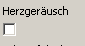
\includegraphics[width=2.2cm]{images/boolfield.png}
\end{center}
\subsubsection{Attribute}
\begin{description}
    \item[default:] Standardwert, wenn die Messung neu erfasst wird (nur
                    \texttt{true} oder \texttt{false} werden akzeptiert)
\end{description}
\subsection{Beispiel}
\begin{lstlisting}
<boolfield name="herger" title="Herzgeraeusch" />
\end{lstlisting}

\subsection{datafield}
Verweis auf andere Messungen
\begin{center}
    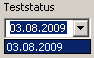
\includegraphics[width=2.6cm]{images/datafield.png}
\end{center}
\subsubsection{Attribute}
\begin{description}
    \item[type:] Name des Messungstyps auf den verwiesen werden soll
\end{description}
\subsection{Beispiel}
\begin{lstlisting}
<datafield  name="vorekg" title="Vorekg" type="ekg" />
\end{lstlisting}

\subsection{calcfield}
Errechnetes Feld
\begin{center}
    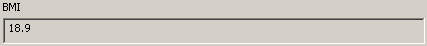
\includegraphics[width=12cm]{images/calcfield.png}
\end{center}
\subsubsection{Attribute}
\begin{description}
    \item[places:] Anzahl der Nachkommastellen beim Ergebnis
\end{description}
\subsubsection{Unterelemente}
Beim calcfield sind 2 verschiedene Unterelemente vorgesehen. Zum einen ist das
\texttt{var}, das es ermöglicht, Felder aus der Messung als Variablen in die
Formel zu importieren, zum andern \texttt{formula}, das die eigentliche Formel
enthält.

Bei \texttt{var} müssen 2 Attribute angegeben werden \texttt{name}, der
Name wie die Variable in der Formel heissen soll, und \texttt{source} mit dem
Feldnamen in der Messung. Bei Datenfeldern kann beispielsweise mit
\texttt{datenfeldname.gewicht} auf das Feld \texttt{gewicht} in der
re\-fe\-ren\-zier\-ten Messung zugegriffen werden. Das ganze kann beliebig tief
verschachtelt werden.

Beim Element \texttt{formula} muss mit dem Attribut \texttt{interpreter} der zu
benutzende Interpreter ausgewählt werden. Im Moment steht jedoch nur «beanshell»
zur Verfügung.
\subsection{Beispiel}
\begin{lstlisting}
<calcfield name="bmi" title="BMI" places="2">
  <var name="gewicht" source="gewicht" />
  <var name="groesse" source="groesse" />
  <formula interpreter="beanshell">
    return gewicht/(groesse*groesse);
  </formula>
</calcfield>
\end{lstlisting}


\section{IDataAccess-Schnittstelle}
Das \texttt{hilotec-messwerte}-Plugin stellt die IDataAccess-Schnittstelle, die
auch von an\-de\-ren Elexis-Plugins benutzt wird, zur Verfügung. Damit wird es unter
anderem auch möglich in Briefen und Berichten auf Werte aus erfassten Messungen
zurückzugreifen. Allgemeine Informationen zu dieser Schnittstelle sind dem
Elexis-Handbuch zu ent\-neh\-men, wo die Schnittstelle genauer beschrieben wird. Im
folgenden soll nur auf den plug\-in\-spe\-zi\-fi\-schen Teil eingegangen werden.

Das Plugin benutzt den Identifier \texttt{Messwerte} fuer die Schnittstelle. Das
heisst, die Platzhalter für den Zugriff haben die Form
\texttt{Messwerte:Patient:auswahl:daten}. Wobei für den Teil \texttt{auswahl} die
folgenden Möglichkeiten bestehen:
\begin{description}
    \item[\texttt{dd.mm.yyyy}:] Messung von genau dem angegebenen Datum
    \item[first:] Erste Messung des Patienten
    \item[last:] Letzte Messnug des Patienten
    \item[firstsince=\texttt{dd.mm.yyyy}:] Erste Messung nach dem angegebenen
                                           Datum
    \item[lastbefore=\texttt{dd.mm.yyyy}:] Letzte Messung vor dem angegebenen
                                           Datum
\end{description}

Der Teil \texttt{daten} hat die Form \texttt{typ.feld}, wobei \texttt{typ} den
Namen des Messungstyp bezeichnet, und \texttt{feld} den Namen des Feldes in dem
Typ. Kommen Datenfelder vor, kann mit einem weiteren Punkt der Feldname in der
referenzierten Messung spezifiziert werden. Auch hier können die Datafelder
wieder beliebig verschachtelt werden.

\section{Layout Steuerung}
Standardmässig wird bei Doppelklick auf eine Messwertreihe ein Dialogfenster geöffnet, welches alle Werte untereinander zum Eingeben und Ändern anbietet. Auf Wunsch kann den einzelnen Messwertreihen aber auch Darstellungsinformation mitgegeben werden. Dies wird gemacht, indem man ein Element $<$design$>$ der $<$datatype$>$ - Definition zufügt.

\end{document}
